\documentclass[tikz,border=10pt,12pt,x11names]{standalone}
\usepackage{tikz}
\usetikzlibrary{circuits.logic.US} % TiKZ Library for US Logic Circuits.
\begin{document}
	\begin{tikzpicture}[circuit logic US,
						tiny circuit symbols,
						every circuit symbol/.style={
						fill=white,draw}]

		\node[draw] at (-2,5) {Module name};

		% Logic Gates in Left Side of Multiplexor
		\node[buffer gate, point down,inputs={i}] (buf1) at (-1,3)    {}; % Input Ea
		\node[and gate,inputs={nnnn}, point down] (and1) at (0,-1)    {};
		\node[and gate,inputs={nnnn}, point down] (and2) at (1.5,-1)  {};
		\node[and gate,inputs={nnnn}, point down] (and3) at (3,-1)    {};
		\node[and gate,inputs={nnnn}, point down] (and4) at (4.5,-1)  {};
		\node[or gate,inputs={nnnn}, point down]  (or1)  at (2.25,-3) {};
		\node[not gate, point down]               (not1) at (5.5,4)   {}; % Input Sa
		\node[buffer gate, point down,inputs={i}] (buf2) at (5.5,2.5) {};
		% Left Side connections
		\draw [red, very thick] (buf1.output) -- ++(down:26.4mm) -| (and1.input 4);
		\draw (and1.output) -- ++(down:5mm) -| (or1.input 4);
		\draw (and2.output) -- ++(down:3mm) -| (or1.input 3);
		\draw (and3.output) -- ++(down:3mm) -| (or1.input 2);
		\draw (and4.output) -- ++(down:5mm) -| (or1.input 1);
		\draw (not1.output) -- (buf2.input);
		% Logic Gates in Right Side of Multiplexor
		\node[not gate, point down] (not2) at (7,4) {}; % Input Sb
		\node[buffer gate, point down,inputs={i}] (buf3) at (7,2.5)    {};
		\node[buffer gate, point down,inputs={i}] (buf4) at (13.50,3)  {}; % Input Eb
		\node[and gate,inputs={nnnn}, point down] (and5) at (8,-1)     {};
		\node[and gate,inputs={nnnn}, point down] (and6) at (9.5,-1)   {};
		\node[and gate,inputs={nnnn}, point down] (and7) at (11,-1)    {};
		\node[and gate,inputs={nnnn}, point down] (and8) at (12.5,-1)  {};
		\node[or gate,inputs={nnnn},  point down] (or2)  at (10.25,-3) {};
		\draw (not2.output) -- (buf3.input);
		% Right Side connections
		\draw [red, very thick] (buf4.output) -- ++(down:26.4mm) -| (and8.input 1);
		\draw (and5.output) -- ++(down:5mm) -|  (or2.input 4);
		\draw (and6.output) -- ++(down:3mm) -|  (or2.input 3);
		\draw (and7.output) -- ++(down:3mm) -|  (or2.input 2);
		\draw (and8.output) -- ++(down:5mm) -|  (or2.input 1);
		% Inputs and Outputs of Multiplexer
		\draw [black,very thick] (buf1.input) -- ++(up:5mm) node [above]{$E_a$};
		    % Enable Signal a
		\draw [black,very thick] (buf4.input) -- ++(up:5mm) node [above]{$E_b$};
		    % Enable Signal b
		\draw [black,very thick] (not1.input) -- ++(up:5mm) node [above]{$S_a$};
		    % Selection Signal a
		\draw [black,very thick] (not2.input) -- ++(up:5mm) node [above]{$S_b$};
		    % Selection Signal b
	 	% Inputs I_na with n={0, 1, 2, 3}
		\draw [black,very thick] (and1.input 1) -- ++(up:4.3) node [above]{$I_{0a}$}; 
		\draw [black,very thick] (and2.input 1) -- ++(up:4.3) node [above]{$I_{1a}$};
		\draw [black,very thick] (and3.input 1) -- ++(up:4.3) node [above]{$I_{2a}$};
		\draw [black,very thick] (and4.input 1) -- ++(up:4.3) node [above]{$I_{3a}$};
		% Inputs I_nb with n={0, 1, 2, 3}
		\draw [black,very thick] (and5.input 4) -- ++(up:4.3) node [above]{$I_{0b}$}; 
		\draw [black,very thick] (and6.input 4) -- ++(up:4.3) node [above]{$I_{1b}$};
		\draw [black,very thick] (and7.input 4) -- ++(up:4.3) node [above]{$I_{2b}$};
		\draw [black,very thick] (and8.input 4) -- ++(up:4.3) node [above]{$I_{3b}$};
		% Output of NOT gates
		\draw [blue, very thick]  (not1.output) -- ++(down:2.5mm)
		      -- ++(left:5mm) -- (5,0.45);
		\draw [blue, very thick]  (not1.output) -- (buf2.input);
		\draw [Gold3, very thick] (not2.output) -- ++(down:2.5mm) -- ++(left:5mm)
		      -- (6.5,0.1);
		\draw [Gold3, very thick] (not2.output) -- (buf3.input);
		% Output of BUFFER gates
		\draw [Brown4, very thick] (buf2.output) -- (5.5,1);
		\draw [Green4, very thick] (buf3.output) -- (7,0.7);
		% Interconnection of AND gates
		\draw [red,very thick]    (and1.input 4) -- ++(up:3mm)  -| (and2.input 4)
		      -- ++(up:3mm) -|    (and3.input 4) -- ++(up:3mm)  -| (and4.input 4);
		\draw [red,very thick]    (and5.input 1) -- ++(up:3mm)  -| (and6.input 1)
		      -- ++(up:3mm) -|    (and7.input 1) -- ++(up:3mm)  -| (and8.input 1);
		\draw [blue,very thick]   (and1.input 3) -- ++(up:9mm)  -| (and2.input 3)
		      -- ++(up:9mm) -|    (and5.input 3) -- ++(up:9mm)  -| (and6.input 3);
		\draw [Gold3,very thick]  (and1.input 2) -- ++(up:6mm)  -| (and3.input 2)
		      -- ++(up:6mm) -|    (and5.input 2) -- ++(up:6mm)  -| (and7.input 2);
		\draw [Green4,very thick] (and2.input 2) -- ++(up:12mm) -| (and4.input 2)
		      -- ++(up:12mm) -|   (and6.input 2) -- ++(up:12mm) -| (and8.input 2);
		\draw [Brown4,very thick] (and3.input 3) -- ++(up:15mm) -| (and4.input 3)
		      -- ++(up:15mm) -|   (and7.input 3) -- ++(up:15mm) -| (and8.input 3);
	    % Outputs of multiplexer
	    % Buffers at output of OR logic gates.
	        \node[buffer gate, point down,inputs={i}] (1y) at (2.25,-4.5)  {};
	        \node[buffer gate, point down,inputs={i}] (2y) at (10.25,-4.5) {};
	    % Connecting output of OR logic gates to Buffers input
	        \draw (or1.output) -- (1y.input);
	        \draw (or2.output) -- (2y.input);
	    % Outputs of multiplexer
		\draw (1y.output) -- ++(down:5mm) node [below]{$1Y$};
		\draw (2y.output) -- ++(down:5mm) node [below]{$2Y$};
	\end{tikzpicture}
	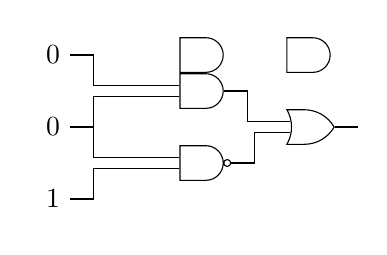
\begin{tikzpicture}[circuit logic US,
						tiny circuit symbols,
						every circuit symbol/.style={
						fill=white,draw}]

		\matrix[column sep=7mm]
		{
			\node (i0) {0}; & &	\node [and gate] (a1) {}; & \node [and gate] (a1) {};\\
							& & \node [and gate] (a1) {};  & \\
			\node (i1) {0}; & &							 & \node [or gate] (o) {};\\
							& & \node [nand gate] (a2) {}; & \\
			\node (i2) {1}; & &							 & \\
		};

		\draw (i0.east) -- ++(right:3mm) |- (a1.input 1);
		\draw (i1.east) -- ++(right:3mm) |- (a1.input 2);
		\draw (i1.east) -- ++(right:3mm) |- (a2.input 1);
		\draw (i2.east) -- ++(right:3mm) |- (a2.input 2);
		\draw (a1.output) -- ++(right:3mm) |- (o.input 1);
		\draw (a2.output) -- ++(right:3mm) |- (o.input 2);
		\draw (o.output) -- ++(right:3mm);

	\end{tikzpicture}
	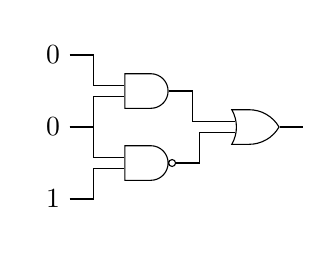
\begin{tikzpicture}[circuit logic US,
						tiny circuit symbols,
						every circuit symbol/.style={
						fill=white,draw}]

		\matrix[column sep=7mm]
		{
			\node (i0) {0}; &							 & \\
							& \node [and gate] (a1) {};  & \\
			\node (i1) {0}; &							 & \node [or gate] (o) {};\\
							& \node [nand gate] (a2) {}; & \\
			\node (i2) {1}; &							 & \\
		};

		\draw (i0.east) -- ++(right:3mm) |- (a1.input 1);
		\draw (i1.east) -- ++(right:3mm) |- (a1.input 2);
		\draw (i1.east) -- ++(right:3mm) |- (a2.input 1);
		\draw (i2.east) -- ++(right:3mm) |- (a2.input 2);
		\draw (a1.output) -- ++(right:3mm) |- (o.input 1);
		\draw (a2.output) -- ++(right:3mm) |- (o.input 2);
		\draw (o.output) -- ++(right:3mm);

	\end{tikzpicture}
\end{document}